\documentclass{examen}

\begin{document}
\modulo{Lenguajes de marcas y sistemas de gesti�n de informaci�n}

Dado el archivo XML que se puede encontrar al final, extraer la informaci�n pedida en los siguientes enunciados usando el lenguaje que se indique

\pregunta{Devolver la media de cantidades suministradas para cada proveedor. Deben salir varias filas como resultado}{2}



\pregunta{Devolver cuantos proyectos reciben alg�n suministro que tenga en cantidad un valor de 650 o m�s. Debe salir un solo resultado.}{2}
\pregunta{Devolver el c�digo de parte y el c�digo de proyecto de la tabla suministra en la que la cantidad sea 300 o menos y adem�s el proveedor sea v1 o v2.}{1}

\pregunta{Devolver la ciudad y el nombre de todos los proveedores cuyo estado sea 10.}{1}


\pregunta{Indicar la ciudad de las partes que reciben una cantidad de 450 o menos.}{1}
\pregunta{Devolver los n�meros de parte y el color de las partes cuyo color sea Azul.}{1}
\pregunta{Devolver la media de peso de las partes por color. Deben salir varios resultados: media de peso para partes cuyo color es Rojo, media de peso para partes cuyo color es Azul, etc...}{2}


\break 
\begin{verbatim}
<datos>
    <proveedores>
        <proveedor numprov="v1">
            <nombreprov>Smith</nombreprov>
            <estado>20</estado>
            <ciudad>Londres</ciudad>
        </proveedor>
        ... omitido ...
    </proveedores>
    <partes>
        <parte numparte="p1">
            <nombreparte>Tuerca</nombreparte>
            <color>Rojo</color>
            <peso>12</peso>
            <ciudad>Londres</ciudad>
        </parte>
        ... omitido ...
    </partes>
    <proyectos>
        <proyecto numproyecto="y1">
            <nombreproyecto>Clasificador</nombreproyecto>
            <ciudad>Paris</ciudad>
        </proyecto>
        ... omitido ...
    </proyectos>
    <suministros>
        <suministra>
            <numprov>v1</numprov>
            <numparte>p1</numparte>
            <numproyecto>y1</numproyecto>
            <cantidad>200</cantidad>
        </suministra>
        <suministra>
            <numprov>v1</numprov>
            <numparte>p1</numparte>
            <numproyecto>y4</numproyecto>
            <cantidad>700</cantidad>
        </suministra>
        ... omitido ...
    </suministros>
</datos>
\end{verbatim}

\begin{figure}[h]
    \caption{Esquema de la base de datos}
    \label{figura1}
    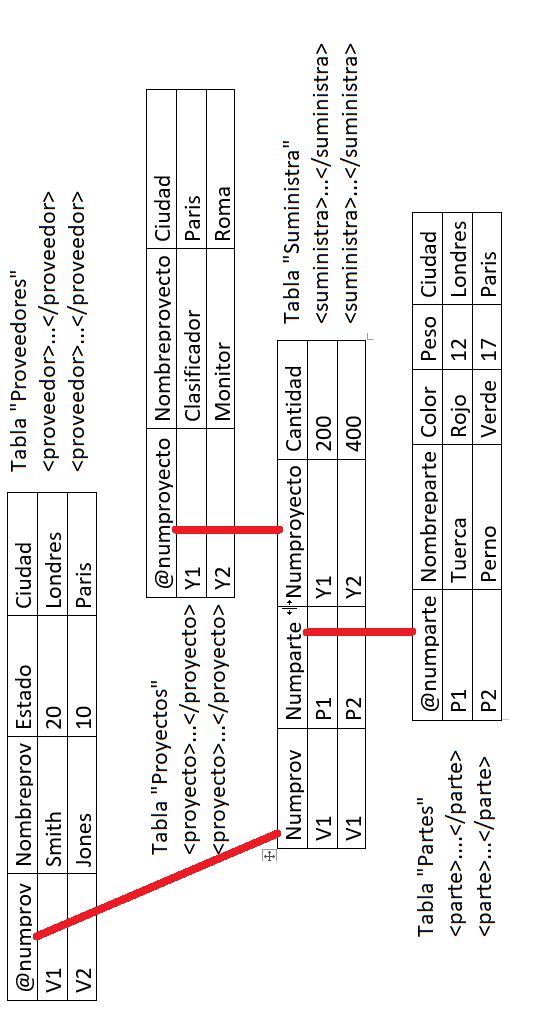
\includegraphics[width=\linewidth]{examen-img/BaseDatosProveedoresPartesProyectos.png}
\end{figure}

\end{document}
